% Provenance (never printed): see sources/outline_sources.md (Year 1: the carbonate factory;
% reefs and platforms; pelagic oozes and the carbonate compensation depth; siliceous oozes;
% evaporite sequences). Exercise and problem values in the Book 3 scratch calculator
% calc/ch22.py; figure data from figdata/bachelor-1/evaporation.py and ccd_flank.py.
% Calcite, aragonite and dolomite are ch. 7's; the depth--age law ch. 13's; salinity Book 1's
% (g8); limestone Book 1's (g6, prose); the carbonate system and alkalinity the chemistry and
% biology books' (recalled, never defined). The subsidence of volcanic islands under reefs is
% the Year 2 volume's (oceanic islands); diagenesis (dolomitisation, chert, gypsum to
% anhydrite) is ch. 23's; upwelling ch. 29's.
\chapter{Sedimentos carbonatados, silíceos y evaporíticos}\label{ch:b1:chemical-biogenic-sediments}

Los acantilados blancos de creta que se miran a través del mar estrecho entre Inglaterra y Francia parecen las rocas más corrientes. Bajo el microscopio electrónico resultan
estar hechos de innumerables placas diminutas de calcita, desprendidas por algas unicelulares que flotaban en el mar que cubría la región. Un \omterm{def:b1:chemical-biogenic-sediments:reef}{arrecife} visto desde una barca es la misma
historia en el otro extremo de la escala: una caliza en formación, construida por corales y algas que toman calcio y carbonato del agua y los convierten en piedra. No todos los sedimentos
son transportados; muchos se forman en el lugar donde yacen, por seres vivos o por el propio agua al evaporarse. Este capítulo sigue las tres grandes familias de estos sedimentos ---
carbonatos, \omterm{def:b1:chemical-biogenic-sediments:ooze}{fangos silíceos} y evaporitas--- desde la química del mar que los alimenta hasta las rocas que dejan.

\begin{recall}
La caliza es una roca sedimentaria formada por calcita, a menudo de conchas, que burbujea en ácido diluido (libro 1, año 6). La calcita y la aragonita son los dos \omterm{def:b1:rock-forming-minerals:polymorph}{polimorfos}
de \ce{CaCO3}, de densidades \qty{2.71}{g.cm^{-3}} y \qty{2.93}{g.cm^{-3}}, y la dolomita \ce{CaMg(CO3)2}, de densidad \qty{2.84}{g.cm^{-3}}, es el carbonato de calcio y
magnesio (\cref{ch:b1:rock-forming-minerals}). La salinidad del agua de mar es la masa de sal disuelta en un kilogramo de ella (libro 1, año 8). En el agua, el dióxido de carbono,
el carbonato de hidrógeno y los iones carbonato están ligados por equilibrios ácido--base, y la alcalinidad mide las bases capaces de captar iones hidrógeno (los libros de química);
el sistema carbonatado del océano participa en el ciclo del carbono (los libros de biología). El fondo marino se hunde con la edad según $d = d_r + C\sqrt t$
(\cref{thm:b1:rifts-ridges-margins:depth-age}).
\end{recall}
% ledger: webmineral:polymorphs, hom:calcite, webmineral:others

\section{La fábrica de carbonato}\label{sec:b1:chemical-biogenic-sediments:factory}

El agua de mar contiene calcio y carbono inorgánico disuelto, sobre todo como carbonato de hidrógeno. El carbonato de calcio se forma a partir de ellos por las reacciones
\[
\ce{Ca^2+ + 2 HCO3- -> CaCO3 + CO2 + H2O}, \qquad
\ce{Ca^2+ + CO3^2- -> CaCO3},
\]
la primera libera una molécula de dióxido de carbono por cada carbonato depositado. El agua superficial cálida de los trópicos está sobresaturada en carbonato de calcio, pero rara vez
precipita por sí sola: casi todo el carbonato lo fabrican seres vivos, que pagan la energía para construir sus conchas y esqueletos y controlan el \omterm{def:b1:rock-forming-minerals:mineral}{mineral} que usan. Los corales y las algas verdes
construyen aragonita; las algas rojas y muchos foraminíferos construyen calcita, parte de ella rica en magnesio; los moluscos usan uno o ambos.

\begin{definition}[Fábrica de carbonato]\label{def:b1:chemical-biogenic-sediments:factory}
La \emph{fábrica de carbonato}\index{fábrica de carbonato} de un mar es el conjunto de organismos y procesos que produce sedimento de carbonato de calcio allí donde se encuentra, en lugar
de traerlo de otro lugar. Sus productos son granos esqueléticos (conchas y esqueletos enteros o rotos), lodo carbonatado, granos recubiertos y los armazones rígidos de los \omterm{def:b1:chemical-biogenic-sediments:reef}{arrecifes}.
\end{definition}

La fábrica más rica trabaja en aguas cálidas, claras, someras e iluminadas por el sol, lejos del lodo de los ríos, que enterraría a los productores y enturbiaría la luz que necesitan las algas.
Su sedimento lo hace el propio fondo marino: restos de coral y de algas, las conchas de los moluscos y de los foraminíferos unicelulares que viven en el fondo, y agujas de aragonita que
desprenden las algas verdes, que se asientan como un lodo de cal. Donde el agua está agitada y sobresaturada, los granos que las olas y las mareas hacen rodar se recubren de capas de carbonato,
una tras otra, alrededor de un núcleo, un grano de arena o un fragmento de concha, hasta formar \omterm{def:b1:chemical-biogenic-sediments:reef}{ooides} redondos
(\cref{def:b1:chemical-biogenic-sediments:reef}). Una segunda fábrica trabaja en el océano abierto, lejos de cualquier costa: el plancton que vive en la capa superficial iluminada construye
pequeñas conchas y placas de calcita que llueven hasta el fondo del mar profundo (\cref{sec:b1:chemical-biogenic-sediments:oozes}).
% ledger: og:carbonates

La rapidez con que construye una fábrica se mide por su presupuesto de carbonato, la masa de carbonato producido y conservado en su sitio cada año sobre un metro cuadrado, después de las
pérdidas por organismos perforadores, ramoneadores y el oleaje. Se convierte en una tasa vertical de crecimiento mediante un balance de masa.

\begin{proposition}[Acreción a partir de un presupuesto de carbonato]\label{prop:b1:chemical-biogenic-sediments:accretion}
Sea un fondo marino que conserva la masa neta $G$ de carbonato de calcio por unidad de área y de tiempo, como un depósito cuyos granos sólidos tienen la densidad $\rho_s$
y cuya porosidad, la fracción de su volumen ocupada por poros, es $\phi$. Entonces el fondo sube a la velocidad
\[
a = \frac{G}{\rho_s\,(1-\phi)}.
\]
\end{proposition}

\begin{proof}
En el tiempo $\mathrm dt$ una unidad de área recibe la masa $G\,\mathrm dt$ de carbonato sólido, que llena el volumen $G\,\mathrm dt/\rho_s$ de granos. Estos granos
forman la fracción $1-\phi$ de la nueva capa, cuyo espesor es, por tanto, $G\,\mathrm dt/(\rho_s(1-\phi))$. Dividiendo por $\mathrm dt$ se obtiene $a$.
\end{proof}

El producto $\rho_s(1-\phi)$ es la densidad aparente seca del depósito. En los \omterm{def:b1:chemical-biogenic-sediments:reef}{arrecifes} del archipiélago de Chagos, en el océano Índico, 28 \omterm{def:b1:chemical-biogenic-sediments:reef}{arrecifes} medidos en 2015 tuvieron un presupuesto
medio de \qty{3.7}{kg} de \ce{CaCO3} por metro cuadrado y por año, y los dominados por corales ramificados de \emph{Acropora} \qty{8.4}{kg}, creciendo unos \qty{4.2}{mm} al año; con la proposición,
estos dos números juntos significan una densidad aparente seca de \qty{2000}{kg.m^{-3}}, es decir, un armazón de \omterm{def:b1:chemical-biogenic-sediments:reef}{arrecife} con cerca de un tercio de espacio poroso
(\cref{exo:b1:chemical-biogenic-sediments:3}). Los mismos \omterm{def:b1:chemical-biogenic-sediments:reef}{arrecifes} habían perdido más de nueve décimas partes de sus corales en el episodio de calentamiento de 1998, y sus presupuestos
muestran lo deprisa que puede reconstruirse un \omterm{def:b1:chemical-biogenic-sediments:reef}{arrecife}.
% ledger: perry:chagos

\section{Arrecifes y plataformas}\label{sec:b1:chemical-biogenic-sediments:reefs}

Donde la fábrica construye un armazón rígido, puede alzarse desde el fondo marino frente a las olas.

\begin{definition}[Arrecife, plataforma carbonatada, ooide]\label{def:b1:chemical-biogenic-sediments:reef}
Un \emph{arrecife}\index{arrecife} es una acumulación carbonatada cuyo armazón de organismos, corales, algas u otros, crecido en el lugar y ligado y cementado entre sí, se alza
sobre el fondo marino circundante y resiste las olas. Una \emph{plataforma carbonatada}\index{plataforma carbonatada} es un cuerpo grueso de carbonato de aguas someras cuya cima plana
yace cerca del nivel del mar y que está limitado por un talud que baja hacia aguas más profundas. Un \emph{ooide}\index{ooide} es un grano redondo del tamaño de la arena formado por capas
concéntricas de carbonato de calcio crecidas alrededor de un núcleo mientras rodaba en agua agitada; una roca hecha de ooides es una oolita.
\end{definition}
% ledger: og:carbonates

Los \omterm{def:b1:chemical-biogenic-sediments:reef}{arrecifes} de coral modernos son de tres clases, nombradas por los navegantes que los cartografiaron mucho antes de que nadie perforara uno. Un \omterm{def:b1:chemical-biogenic-sediments:reef}{arrecife} \emph{frangente}
está unido a la orilla de una isla o de un continente. Un \omterm{def:b1:chemical-biogenic-sediments:reef}{arrecife} \emph{barrera} está separado de la tierra por una laguna, que puede ser ancha y tener decenas de metros de
profundidad: la barrera del nordeste de Australia recorre, con interrupciones, casi mil millas, encerrando un mar de 10 a 25 brazas de profundidad, unos 18 a \qty{46}{m}. Un
\emph{atolón} es un anillo de \omterm{def:b1:chemical-biogenic-sediments:reef}{arrecife}, con islas bajas de arena coralina, alrededor de una laguna que no tiene tierra en absoluto.

\begin{omfigure}
\begin{tikzpicture}[font=\footnotesize, scale=0.72]
% three reef types in cross-section (schematic): a volcanic cone y = 2 - s - 0.75|x - 4|
% subsided by s (0, 0.8, 1.6), sea level at y = 1; the reef grows up from its first
% position, the foot of the fringing reef at (2, 0.5) moving down with the cone
\foreach \s/\yo/\lab/\name in {0/0/a/arrecife frangente, 0.8/-3.8/b/arrecife barrera, 1.6/-7.6/c/atolón} {
  \begin{scope}[yshift=\yo cm]
    \begin{scope}
      \clip (0,-1.3) rectangle (8,2.3);
      \fill[omSea] (0,-1.3) rectangle (8,1.0);
      \draw[lith basalt] (-1,2-\s-3.75) -- (4,2-\s) -- (9,2-\s-3.75) -- cycle;
    \end{scope}
    \draw[omSea!60!black] (0,1.0) -- (8,1.0);
    \node[anchor=west, font=\scriptsize] at (8.05,1.0) {nivel marino};
    \node[anchor=west] at (0,2.05) {(\lab) \name};
    \draw[black!70] (1.05,1.55) node[anchor=east, font=\scriptsize] {arrecife} -- (2.2,1.02);
  \end{scope}
}
% (a) fringing reef: wedges against the shore
\fill[lith reef limestone, draw=black!70] (2.0,0.5) -- (2.15,1.0) -- (2.667,1.0) -- cycle;
\fill[lith reef limestone, draw=black!70] (6.0,0.5) -- (5.85,1.0) -- (5.333,1.0) -- cycle;
\node[anchor=west, font=\scriptsize] at (4.9,1.75) {isla volcánica};
% (b) barrier reef: the cone has sunk by 0.8, the reef has grown up, a lagoon opens
\begin{scope}[yshift=-3.8cm]
  \fill[lith reef limestone, draw=black!70] (2.0,-0.3) -- (2.15,1.0) -- (2.6,1.0) -- (2.55,0.1125) -- cycle;
  \fill[lith reef limestone, draw=black!70] (6.0,-0.3) -- (5.85,1.0) -- (5.4,1.0) -- (5.45,0.1125) -- cycle;
  \draw[black!70] (3.2,0.85) -- (3.45,1.55) node[anchor=south west, font=\scriptsize, inner sep=1pt] {laguna};
\end{scope}
% (c) atoll: the cone has sunk by 1.6 and is drowned; the reef ring encloses a lagoon
\begin{scope}[yshift=-7.6cm]
  \fill[lith limestone, draw=black!50] (2.55,-0.6875) -- (2.55,0.55) -- (5.45,0.55) -- (5.45,-0.6875) -- (4,0.4) -- cycle;
  \fill[lith reef limestone, draw=black!70] (2.0,-1.1) -- (2.15,1.0) -- (2.6,1.0) -- (2.55,-0.6875) -- cycle;
  \fill[lith reef limestone, draw=black!70] (6.0,-1.1) -- (5.85,1.0) -- (5.4,1.0) -- (5.45,-0.6875) -- cycle;
  \node[font=\scriptsize] at (4,0.78) {laguna};
  \node[font=\scriptsize, fill=omLithLime, inner sep=1pt] at (4,0.05) {sedimento lagunar};
\end{scope}
% photograph
\node[anchor=north west, inner sep=0] at (10.75,2.3) {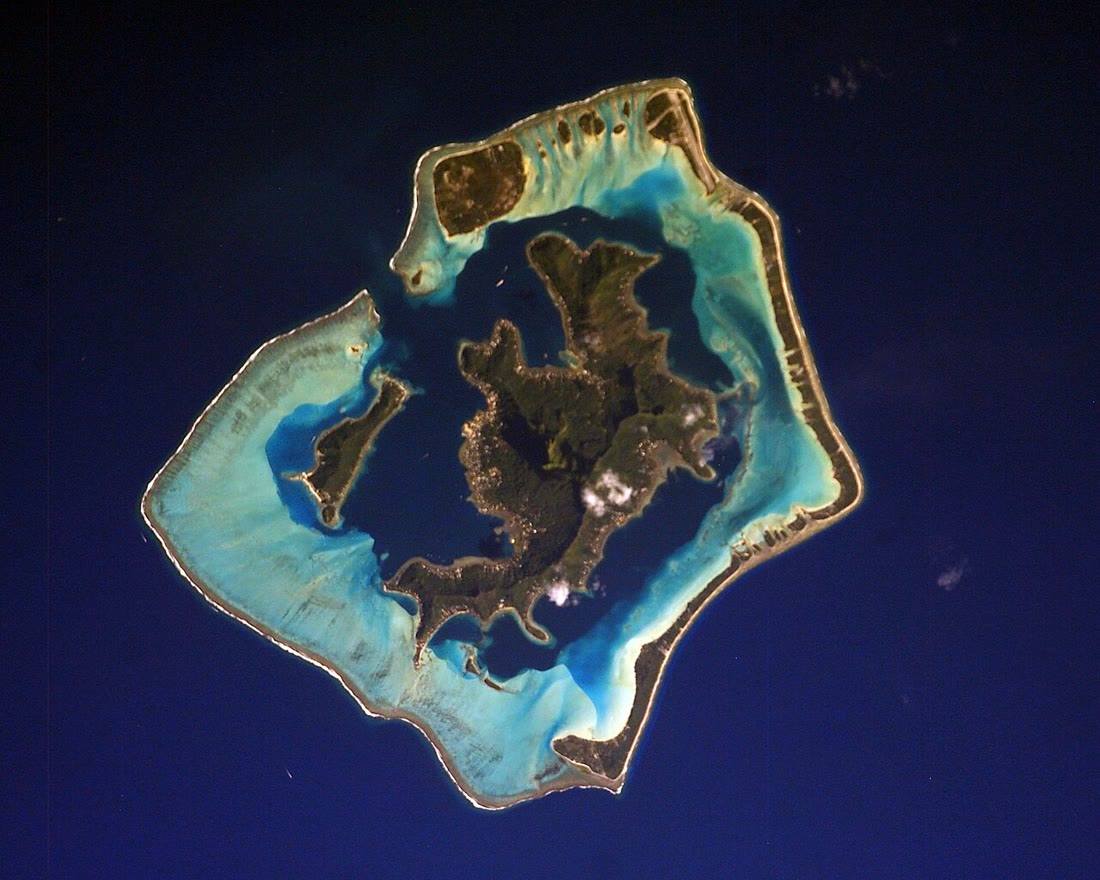
\includegraphics[height=6.6cm]{images/book3/b1-bora-bora.jpg}};
\end{tikzpicture}

{\small Izquierda: los tres tipos de \omterm{def:b1:chemical-biogenic-sediments:reef}{arrecife} de coral en corte transversal (esquemático, con la escala vertical muy exagerada), dibujados como los explicó Darwin: (a)~un \omterm{def:b1:chemical-biogenic-sediments:reef}{arrecife}
que orla una isla volcánica; (b)~la isla se ha hundido y el \omterm{def:b1:chemical-biogenic-sediments:reef}{arrecife}, que crece hacia arriba, se ha convertido en una barrera separada de la orilla por una laguna; (c)~la isla se ha
hundido fuera de la vista y el \omterm{def:b1:chemical-biogenic-sediments:reef}{arrecife} es un atolón alrededor de una laguna cuyo fondo es sedimento carbonatado. Derecha: Bora Bora, una isla volcánica en una laguna encerrada por una
barrera de \omterm{def:b1:chemical-biogenic-sediments:reef}{arrecife} con islas bajas encima, fotografiada por un astronauta desde la Estación Espacial Internacional el 19 de marzo de 2003 (NASA, dominio público, a través de
Wikimedia Commons).}
\label{fig:b1:chemical-biogenic-sediments:reefs}
\end{omfigure}
% ledger: darwin:reefs, commons:bora-bora

\begin{history}[Arrecifes sobre cimientos que se hunden, 1837--1842]
Durante el viaje del \emph{Beagle}, Charles Darwin navegó entre los \omterm{def:b1:chemical-biogenic-sediments:reef}{arrecifes} del Pacífico y del Índico. Razonó a partir de un hecho: los corales constructores de \omterm{def:b1:chemical-biogenic-sediments:reef}{arrecifes}, concluyó,
no prosperan en los casos ordinarios más profundo que entre 20 y 30 brazas, unos 37 a \qty{55}{m}. Sin embargo, las barreras y los atolones se alzan desde aguas profundas, muy por
debajo de ese límite. Sus cimientos, argumentó, deben haberse hundido, lo bastante despacio para que los corales mantuvieran sus cimas en la superficie creciendo hacia arriba: un
\omterm{def:b1:chemical-biogenic-sediments:reef}{arrecife} que orla una isla volcánica se convierte en barrera a medida que la isla se hunde dentro de él, y en atolón cuando la isla ha desaparecido. Leyó su teoría ante la Sociedad
Geológica de Londres el 31 de mayo de 1837 y la publicó en 1842 en \emph{The Structure and Distribution of Coral Reefs}, con un mapa de todos los \omterm{def:b1:chemical-biogenic-sediments:reef}{arrecifes} del mundo clasificados en los tres
tipos. Por qué se hunden las islas oceánicas, y cuánto, es asunto del enfriamiento de la placa que yace bajo ellas, tratado en el volumen del año~2.
\end{history}
% ledger: darwin:reefs

Un \omterm{def:b1:chemical-biogenic-sediments:reef}{arrecife} sobrevive solo si su cima se mantiene en el agua somera donde viven sus constructores. El nivel del mar cambia, y el cimiento puede hundirse; lo que importa es la suma de
los dos, la subida relativa del nivel del mar.

\begin{proposition}[Seguir el ritmo o ahogarse]\label{prop:b1:chemical-biogenic-sediments:keep-up}
Sea la cima de un \omterm{def:b1:chemical-biogenic-sediments:reef}{arrecife} situada a la profundidad $D_0$ bajo el nivel del mar y que crece hacia arriba a la velocidad $a$, mientras el nivel relativo del mar sube a la velocidad $r$,
ambas constantes. Entonces la profundidad del agua sobre el \omterm{def:b1:chemical-biogenic-sediments:reef}{arrecife} tras el tiempo $t$ es
\[
D(t) = D_0 + (r - a)\,t .
\]
Si $a \ge r$, el \omterm{def:b1:chemical-biogenic-sediments:reef}{arrecife} sigue el ritmo del mar (cuando $a > r$ su cima alcanza la superficie, y desde entonces solo puede crecer lateralmente); si $a < r$ se queda atrás, y si sus constructores
no pueden vivir más profundo que $D_{\max}$, se ahoga tras el tiempo $(D_{\max} - D_0)/(r - a)$.
\end{proposition}

\begin{proof}
Mídanse las alturas hacia arriba desde una marca fija en el cimiento. La cima del \omterm{def:b1:chemical-biogenic-sediments:reef}{arrecife} está en $h_0 + a t$ y la superficie del mar en $s_0 + r t$, así que la profundidad del agua
sobre la cima es $D = (s_0 - h_0) + (r - a)t = D_0 + (r-a)t$. Cuando $a > r$, $D$ llega a cero en $t = D_0/(a-r)$ y el \omterm{def:b1:chemical-biogenic-sediments:reef}{arrecife} no puede crecer por encima del mar. Cuando
$a < r$, $D$ crece linealmente y alcanza $D_{\max}$ cuando $(r-a)t = D_{\max} -
D_0$.
\end{proof}

Un \omterm{def:b1:chemical-biogenic-sediments:reef}{arrecife} cuya cima se ha ahogado no muere de inmediato, pero la luz se atenúa, los constructores cambian y la fábrica se frena, de modo que un \omterm{def:b1:chemical-biogenic-sediments:reef}{arrecife} que empieza a quedarse atrás se
queda atrás más aún: los \omterm{def:b1:chemical-biogenic-sediments:reef}{arrecifes} y plataformas ahogados, cubiertos por sedimentos de aguas profundas, se encuentran en los taludes de muchas islas oceánicas y en el registro de las rocas.

A lo largo de millones de años, las fábricas construyen \omterm{def:b1:chemical-biogenic-sediments:reef}{plataformas carbonatadas}, cuerpos gruesos de carbonato de aguas someras que crecen a medida que sus cimientos se hunden. Se repiten
dos formas (véase la figura de abajo). Una \emph{plataforma con borde} tiene una cima plana, protegida tras un borde de \omterm{def:b1:chemical-biogenic-sediments:reef}{arrecifes} y bancos de \omterm{def:b1:chemical-biogenic-sediments:reef}{ooides} en su extremo, que rompe las olas; detrás
de ella yace una laguna tranquila de lodo de cal, y delante un talud empinado por el que caen a la cuenca bloques y derrubios desprendidos del borde. Una \emph{rampa} baja muy suavemente desde la
orilla hacia la cuenca sin ruptura: bancos de \omterm{def:b1:chemical-biogenic-sediments:reef}{ooides} y bancos de conchas donde las olas agitan el fondo, luego lechos de restos de conchas barridos por las tormentas, y luego lodo de cal por
debajo del alcance de las olas. Una plataforma con borde crece sobre todo hacia arriba y hacia afuera desde su borde; una rampa, desplazando sus cinturones de sedimento hacia la costa o hacia el mar
a medida que el mar sube o baja.

\begin{omfigure}
\begin{tikzpicture}[font=\footnotesize, >={Stealth[length=4pt]}]
% (a) rimmed shelf and (b) ramp, schematic cross-sections
\begin{scope}
  \fill[omSea] (0,0.2) rectangle (7.2,2.0);
  \fill[lith limestone, draw=black!60] (0,0) -- (0,1.55) -- (4.3,1.55) -- (4.5,1.75) -- (4.9,1.75) -- (5.1,1.5) -- (6.4,0.35) -- (7.2,0.3) -- (7.2,0) -- cycle;
  \fill[lith reef limestone, draw=black!70] (4.3,1.55) -- (4.5,1.75) -- (4.9,1.75) -- (5.1,1.5) -- (4.8,1.05) -- (4.3,1.05) -- cycle;
  \draw[omSea!60!black] (0,2.0) -- (7.2,2.0);
  \node at (2.1,1.78) {laguna: lodo de cal};
  \node[anchor=south, align=center, font=\scriptsize] at (4.7,2.05) {borde de arrecife y\\ bancos de ooides};
  \node[anchor=west, font=\scriptsize] at (5.6,1.2) {talud: derrubios};
  \node[font=\scriptsize] at (6.75,0.75) {cuenca};
  \node at (3.6,-0.35) {(a) plataforma con borde};
\end{scope}
\begin{scope}[xshift=8.0cm]
  \fill[omSea] (0,0.2) rectangle (7.2,2.0);
  \fill[lith limestone, draw=black!60] (0,0) -- (0,1.85) -- (7.2,0.55) -- (7.2,0) -- cycle;
  \draw[omSea!60!black] (0,2.0) -- (7.2,2.0);
  \draw[densely dashed, black!50] (0,1.6) -- (7.2,1.6) node[pos=1, anchor=south east, font=\scriptsize, inner sep=1pt] {alcanzan las olas de buen tiempo};
  \draw[densely dashed, black!50] (0,1.0) -- (7.2,1.0) node[pos=1, anchor=south east, font=\scriptsize, inner sep=1pt] {alcanzan las olas de tormenta};
  \node[anchor=south, font=\scriptsize] at (0.9,2.05) {bancos de ooides};
  \node[anchor=south, font=\scriptsize] at (3.4,2.05) {lechos de conchas de tormenta};
  \node[anchor=south, font=\scriptsize] at (6.1,2.05) {lodo de cal};
  \node at (3.6,-0.35) {(b) rampa};
\end{scope}
\end{tikzpicture}

{\small Las dos formas de \omterm{def:b1:chemical-biogenic-sediments:reef}{plataforma carbonatada} (esquemáticas, pendientes muy exageradas). (a)~Una plataforma con borde: un borde de \omterm{def:b1:chemical-biogenic-sediments:reef}{arrecifes} y bancos de \omterm{def:b1:chemical-biogenic-sediments:reef}{ooides} rompe las
olas, detrás de él yace una laguna tranquila de lodo de cal, y los derrubios desprendidos del borde caen por el talud hacia la cuenca. (b)~Una rampa baja suavemente desde la
orilla hacia la cuenca, con sus sedimentos clasificados por la profundidad que alcanzan las olas.}
\label{fig:b1:chemical-biogenic-sediments:platforms}
\end{omfigure}

\section{Fangos pelágicos y profundidad de compensación del carbonato}\label{sec:b1:chemical-biogenic-sediments:oozes}

Lejos de la tierra, el fondo marino recibe casi nada de los continentes salvo el polvo eólico más fino. Lo que cae sobre él son, en cambio, los esqueletos del plancton que vivió en
el agua iluminada por el sol, kilómetros más arriba: las placas de calcita de los cocolitofóridos y las conchas de los foraminíferos, las frústulas de ópalo de las diatomeas y los
esqueletos de los radiolarios (representados un poco más adelante). La lluvia prolongada de cocolitos hasta el fondo del mar es el proceso principal que forma la creta y gran parte
de la caliza del mundo.
% ledger: nasa:coccoliths-b3, og:carbonates

\begin{definition}[Fango calcáreo, fango silíceo]\label{def:b1:chemical-biogenic-sediments:ooze}
Un fango es un sedimento pelágico de grano fino, depositado en el océano abierto, formado sobre todo por esqueletos de plancton. Es un \emph{fango calcáreo}\index{fango calcáreo} cuando sus
esqueletos son de carbonato de calcio, sobre todo cocolitos y foraminíferos, y un \emph{fango silíceo}\index{fango silíceo} cuando son de ópalo, sílice amorfa hidratada, sobre todo diatomeas y radiolarios.
\end{definition}
% ledger: og:carbonates

Los \omterm{def:b1:chemical-biogenic-sediments:ooze}{fangos calcáreos} cubren cerca de la mitad del fondo marino del mundo, pero solo por encima de cierta profundidad: por debajo de unos \qty{4500}{m} desaparecen. Las conchas no
dejan de caer allí; se disuelven. El océano profundo es frío y la presión es alta, y la solubilidad de la calcita aumenta con la profundidad, sobre todo por la presión, mientras que la
concentración de iones carbonato en el agua disminuye en general con la profundidad (la química de estos equilibrios se recuerda de los libros de química). Por debajo de cierta profundidad el
agua profunda está subsaturada en calcita, y las conchas que llegan al fondo se disuelven tanto más deprisa cuanto más hondo yacen.
% ledger: britannica:ccd, slotnick:ccd-definitions

\begin{omfigure}
\begin{tikzpicture}
\node[inner sep=0] (a) at (0,0) {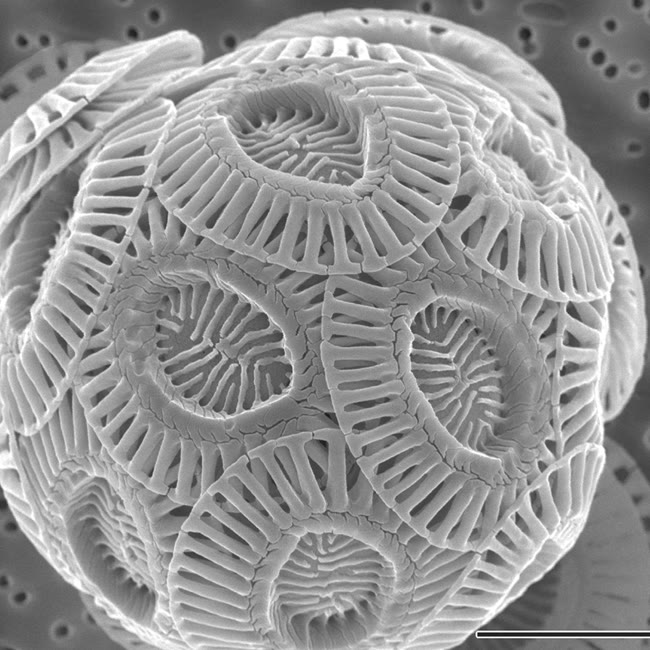
\includegraphics[height=4.3cm]{images/book3/b1-coccolithophore.jpg}};
\node[inner sep=0, anchor=west] (b) at ([xshift=0.25cm]a.east) {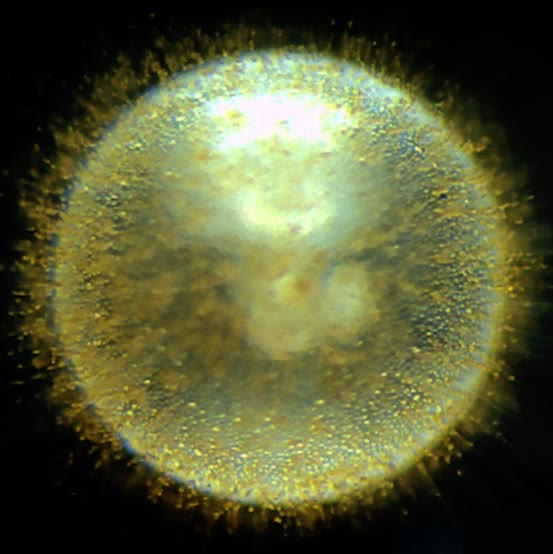
\includegraphics[height=4.3cm]{images/book3/b1-orbulina.jpg}};
\node[inner sep=0, anchor=west] (c) at ([xshift=0.25cm]b.east) {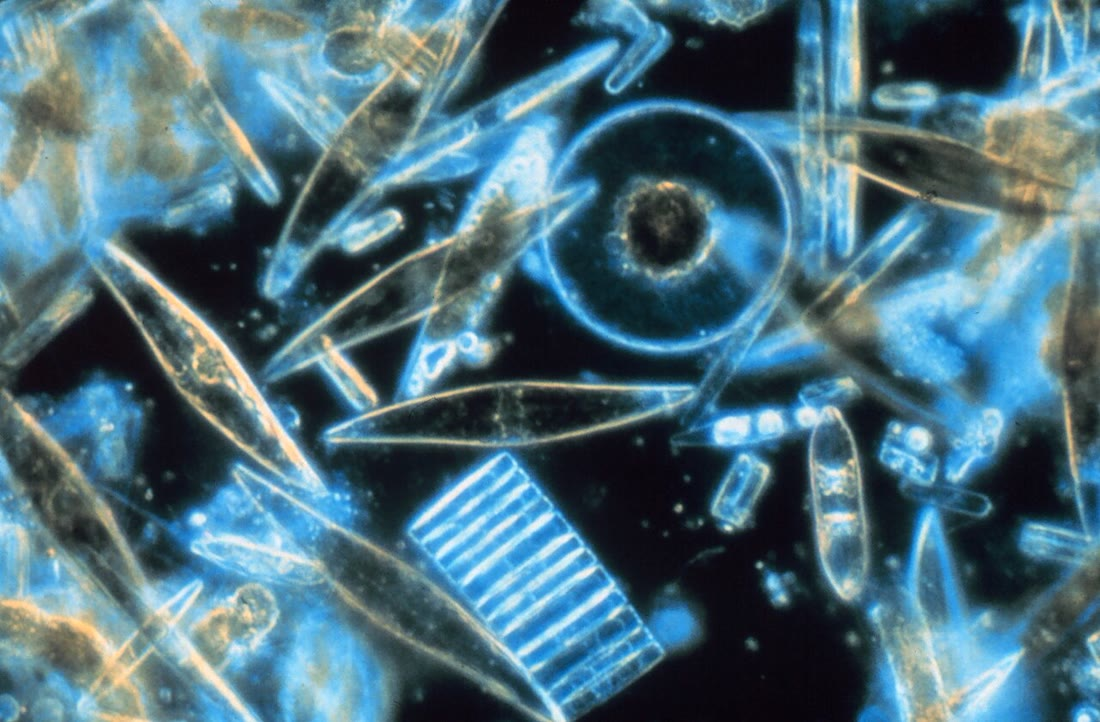
\includegraphics[height=4.3cm]{images/book3/b1-diatoms.jpg}};
\node[font=\footnotesize, anchor=north] at (a.south) {(a) un cocolitofórido};
\node[font=\footnotesize, anchor=north] at (b.south) {(b) un foraminífero};
\node[font=\footnotesize, anchor=north] at (c.south) {(c) diatomeas};
\end{tikzpicture}

{\small Los fabricantes de fangos. (a)~Una sola célula de \emph{Emiliania huxleyi}, blindada con cocolitos, sus placas de calcita (microscopio electrónico de barrido; Alison R.~Taylor,
Universidad de Carolina del Norte en Wilmington, CC~BY~2.5, a través de Wikimedia Commons). (b)~Un foraminífero planctónico vivo, \emph{Orbulina universa}, con su concha de calcita rodeada
de espinas (microscopio óptico; H.~Takagi y coautores, 2019, CC~BY~4.0, a través de Wikimedia Commons). (c)~Diatomeas vivas del hielo marino del estrecho de McMurdo, Antártida, cada una en su
frústula de ópalo (microscopio óptico; Gordon T.~Taylor, Universidad de Stony Brook, NOAA, dominio público, a través de Wikimedia Commons).}
\label{fig:b1:chemical-biogenic-sediments:plankton}
\end{omfigure}
% ledger: commons:ehux, commons:orbulina, commons:diatoms-noaa

\begin{definition}[Lisoclina, profundidad de compensación del carbonato]\label{def:b1:chemical-biogenic-sediments:ccd}
La \emph{lisoclina}\index{lisoclina} es la profundidad del océano por debajo de la cual la disolución de la calcita en el fondo marino se hace visible por primera vez en el sedimento
y su tasa aumenta bruscamente. La \emph{profundidad de compensación del carbonato}\index{profundidad de compensación del carbonato} (CCD) es la profundidad a la que la tasa de disolución
de la calcita iguala la tasa a la que la calcita llueve sobre el fondo marino; por debajo de ella no se acumula carbonato de calcio. En la práctica se sitúa donde el contenido de carbonato de calcio
del sedimento superficial baja por debajo del \qty{10}{\%} en peso.
\end{definition}
% ledger: slotnick:ccd-definitions

La CCD yace en general cientos de metros por debajo de la \omterm{def:b1:chemical-biogenic-sediments:ccd}{lisoclina}. No es un nivel fijo: lo fija un equilibrio entre aporte y disolución, de modo que yace más hondo donde el plancton produce más
carbonato y donde el agua profunda es menos corrosiva. En el Atlántico yace unos \qty{500}{m} más hondo que en el Pacífico, resultado a la vez de un aporte mayor de carbonato y de una disolución más
lenta; solo en el Pacífico occidental yace a unos \qty{4000}{m} en el noroeste y a unos \qty{5100}{m} en el Pacífico central. La aragonita, más soluble que la calcita, se disuelve a profundidades aún
menores. A lo largo del tiempo geológico, los cambios en el aporte, en la productividad y en la disolución han desplazado la CCD más de \qty{2000}{m}.
% ledger: slotnick:ccd-definitions, britannica:ccd, zhang:ccd-west-pacific

\begin{method}[Localizar la lisoclina y la CCD]\label{met:b1:chemical-biogenic-sediments:ccd}
\begin{enumerate}
  \item Recójanse los primeros centímetros de sedimento en lugares de distintas profundidades de una misma región, lo bastante lejos de la tierra y de las zonas de surgencia para que la dilución por arcilla o por ópalo sea pequeña.
  \item Mídase el porcentaje en peso de \ce{CaCO3} de cada muestra y represéntese frente a la profundidad del agua.
  \item La \omterm{def:b1:chemical-biogenic-sediments:ccd}{lisoclina} es la profundidad donde el contenido empieza a bajar bruscamente, y donde las conchas muestran las primeras señales de disolución (foraminíferos rotos y grabados).
  \item La CCD es la profundidad donde el contenido baja al \qty{10}{\%}: léase por interpolación lineal entre las dos muestras a uno y otro lado.
\end{enumerate}
\end{method}

En el flanco de una dorsal oceánica, el fondo marino es joven y somero cerca del eje, y se hunde a medida que envejece y se aleja. Un trozo de fondo nacido por encima de la CCD acumula \omterm{def:b1:chemical-biogenic-sediments:ooze}{fango
calcáreo} hasta que se hunde por debajo de la CCD; desde entonces recibe solo lo que no se disuelve: el polvo que cae del aire, óxidos de hierro y manganeso, los dientes de los peces. Este depósito
lento y pardo es la arcilla roja de las cuencas profundas.

\begin{proposition}[Cruzar la CCD]\label{prop:b1:chemical-biogenic-sediments:flank}
Sea el fondo marino de edad $t$ situado a la profundidad $d(t) = d_r + C\sqrt t$
(\cref{thm:b1:rifts-ridges-margins:depth-age}), con un eje de dorsal a la profundidad $d_r$
más somera que una \omterm{def:b1:chemical-biogenic-sediments:ccd}{profundidad de compensación del carbonato} $z_c$ que permanece constante. Entonces
\[
t_c = \left(\frac{z_c - d_r}{C}\right)^2 ,
\]
y un emplazamiento de edad $t > t_c$ contiene, de abajo arriba, la \omterm{def:b1:layered-earth:layers}{corteza} volcánica, el \omterm{def:b1:chemical-biogenic-sediments:ooze}{fango calcáreo} depositado durante el tiempo $t_c$, y la arcilla roja depositada durante el
tiempo $t - t_c$.
\end{proposition}

\begin{proof}
La profundidad $d(t)$ aumenta con $t$, y $d(t_c) = z_c$ da $C\sqrt{t_c} =
z_c - d_r$, de donde $t_c$. Antes de $t_c$ el fondo yace por encima de la CCD, donde la calcita llueve más
deprisa de lo que se disuelve y se acumula fango; después de $t_c$ yace por debajo, donde no se acumula carbonato y solo se añade arcilla insoluble. El fango, una vez enterrado bajo la arcilla,
queda protegido del agua corrosiva de encima, así que el orden de las capas es el de los tiempos.
\end{proof}

Con $d = 2500 + 350\sqrt t$ (metros, $t$ en millones de años), una CCD a \qty{4500}{m} se cruza a la edad $(2000/350)^2 = \qty{32.7}{Myr}$; a una \omterm{def:b1:plate-kinematics:spreading-rate}{velocidad de expansión
media} de \qty{25}{mm} al año, eso son \qty{816}{km} del eje (figura de abajo). Al perforar un fondo oceánico antiguo se encuentra este orden una y otra vez: basalto, luego \omterm{def:b1:chemical-biogenic-sediments:ooze}{fango calcáreo} o creta,
luego arcilla roja, un registro del viaje del fondo por el flanco. Donde la placa se ha desplazado después bajo un cinturón de alta productividad, cerca del ecuador, la arcilla puede quedar
cubierta por una nueva capa de fango, y así los testigos registran el movimiento de las placas además de la profundidad de la CCD.
% ledger: parsons:plate-model

\begin{omfigure}
\begin{tikzpicture}[font=\footnotesize]
\begin{axis}[width=11cm, height=5.6cm, xmin=0, xmax=1750, ymin=2000, ymax=6200, y dir=reverse,
    xlabel={distancia al eje de la dorsal (km), velocidad de expansión media \qty{25}{mm.yr^{-1}}},
    ylabel={profundidad (m)}, ytick={2000,3000,...,6000},
    axis on top, clip=false]
  % sea water above the floor
  \addplot[fill=omSea, draw=none] table[x=x_km, y=depth] {figdata/out/bachelor-1-ccd_flank-profile.dat} -- (axis cs:1750,2000) -- (axis cs:0,2000) -- cycle;
  % floor: ooze-covered above the CCD, red clay below
  \addplot[very thick, draw=omLithLime!70!black, restrict x to domain=0:816.3] table[x=x_km, y=depth] {figdata/out/bachelor-1-ccd_flank-profile.dat};
  \addplot[very thick, draw=brown!70!black, restrict x to domain=816.3:1750] table[x=x_km, y=depth] {figdata/out/bachelor-1-ccd_flank-profile.dat};
  \draw[thick, omThm, densely dashed] (axis cs:0,4500) -- (axis cs:1750,4500) node[pos=0.99, anchor=north east, inner sep=1.5pt] {CCD, \qty{4500}{m}};
  \draw[black!60, dotted, thick] (axis cs:0,4050) -- (axis cs:1750,4050) node[pos=0.99, anchor=south east, inner sep=1.5pt] {lisoclina (esquemática)};
  \fill[omThm] (axis cs:816.3,4500) circle[radius=2pt];
  \node[anchor=north east, align=right] at (axis cs:790,4620) {el fondo cruza la CCD\\ a \qty{32.7}{Myr}, \qty{816}{km}};
  \node[anchor=north, align=center, omLithLime!40!black] at (axis cs:520,2750) {se acumula\\ fango calcáreo};
  \node[anchor=north west, align=left, brown!60!black] at (axis cs:1000,5180) {arcilla roja sobre\\ fango enterrado};
\end{axis}
% sediment column at the site 1500 km from the axis (60 Myr), schematic
\begin{scope}[xshift=10.6cm, yshift=0.4cm]
  \draw[lith basalt] (0,0) rectangle (0.9,1.0);
  \draw[lith limestone] (0,1.0) rectangle (0.9,2.6);
  \fill[brown!45, draw=black!60] (0,2.6) rectangle (0.9,3.2);
  \node[anchor=west, align=left, font=\scriptsize] at (1.0,0.5) {corteza basáltica};
  \node[anchor=west, align=left, font=\scriptsize] at (1.0,1.8) {fango calcáreo\\ (0 a \qty{32.7}{Myr})};
  \node[anchor=west, align=left, font=\scriptsize] at (1.0,2.9) {arcilla roja};
  \node[anchor=south, font=\scriptsize, align=center] at (0.9,3.3) {columna a \qty{1500}{km}\\ (esquemática)};
\end{scope}
\end{tikzpicture}

{\small Sedimentos pelágicos en el flanco de una dorsal. El fondo se hunde con la edad según la ley de profundidad--edad $d = 2500 + 350\sqrt t$ y se aleja del eje a
\qty{25}{mm} al año; por encima de la \omterm{def:b1:chemical-biogenic-sediments:ccd}{profundidad de compensación del carbonato}, situada aquí en \qty{4500}{m}, acumula \omterm{def:b1:chemical-biogenic-sediments:ooze}{fango calcáreo}; por debajo, solo arcilla roja. Un
emplazamiento alejado del eje lleva basalto, fango y arcilla roja, de abajo arriba (columna de la derecha, espesores esquemáticos). La \omterm{def:b1:chemical-biogenic-sediments:ccd}{lisoclina}, dibujada unos cientos de metros
por encima de la CCD, marca donde empieza a notarse la disolución.}
\label{fig:b1:chemical-biogenic-sediments:flank}
\end{omfigure}
% computed in figdata/bachelor-1/ccd_flank.py; ledger: parsons:plate-model, britannica:ccd, slotnick:ccd-definitions

\section{Fango silíceos y sílex}\label{sec:b1:chemical-biogenic-sediments:silica}

Las diatomeas, algas unicelulares del plancton, y los radiolarios, miembros unicelulares del zooplancton, construyen sus esqueletos de ópalo, que toman del ácido silícico disuelto en el agua
de mar. A diferencia de la calcita de la superficie del océano, el ópalo no está protegido por la sobresaturación: el agua de mar está subsaturada en él a todas las profundidades, y la mayor parte
del ópalo se disuelve en cuanto muere el organismo, primero en el agua al hundirse y luego en el fondo marino. De los \num{255}~teramoles de silicio que el plancton del océano mundial incorpora
cada año al ópalo, solo unos 9.2 quedan enterrados para siempre en el sedimento: una conservación de un \qty{3.6}{\%}. Un átomo de silicio que el río lleva al mar es captado y liberado de nuevo por el
plancton unas dieciséis veces antes de quedar enterrado, y permanece unos \num{8000} años en el océano.
% ledger: treguer:silica

Así, los \omterm{def:b1:chemical-biogenic-sediments:ooze}{fangos silíceos} se forman donde la producción de ópalo es tan alta que incluso el \qty{3.6}{\%} se suma, y donde casi nada más lo diluye: alrededor del océano Austral, en el Pacífico norte, a lo
largo del ecuador en el Pacífico y en los márgenes continentales, los lugares donde el agua profunda rica en nutrientes asciende a la superficie (\cref{ch:b1:ocean-circulation}). También dominan
por debajo de la CCD bajo aguas productivas, donde la calcita que cayó con ellos se ha disuelto.
% ledger: treguer:silica, og:carbonates

\begin{definition}[Sílex]\label{def:b1:chemical-biogenic-sediments:chert}
Un \emph{sílex}\index{sílex} es una roca sedimentaria dura y densa de cuarzo microcristalino, formada en la mayoría de los casos a partir de ópalo biogénico que se disolvió y recristalizó tras el
enterramiento; aparece en capas, a menudo procedentes de \omterm{def:b1:chemical-biogenic-sediments:ooze}{fangos silíceos}, o en nódulos, de los cuales el pedernal, en la creta, es el mejor conocido.
\end{definition}
% ledger: og:carbonates

Un fango de diatomeas que no se ha recristalizado se convierte en diatomita, una roca ligera, blanca y porosa, casi ópalo puro. Con el enterramiento y el tiempo el ópalo se convierte en otras formas
de sílice y, por último, en cuarzo, y la sílice migra: abandona la creta, por ejemplo, y se reúne en nódulos de pedernal a lo largo de ciertas capas. Cómo ocurre esto corresponde a la diagénesis
(\cref{ch:b1:diagenesis-basins}).

\section{Evaporitas}\label{sec:b1:chemical-biogenic-sediments:evaporites}

Donde una masa de agua de mar pierde más agua por evaporación de la que recibe, sus sales se concentran hasta precipitar una tras otra. La composición del agua de mar es la misma, en sus iones
mayoritarios, en todos los océanos (\cref{tab:b1:chemical-biogenic-sediments:seawater}).
(\cref{tab:b1:chemical-biogenic-sediments:seawater}).

\begin{table}[htbp]
\centering\small
\begin{tabular}{@{}lrrr@{}}
\hline
ion & fracción másica de la sal marina & \si{g} por \si{kg} de agua de mar & \si{mmol} por \si{kg} \\
\hline
cloruro \ce{Cl-} & 0.5503 & 19.353 & 545.9 \\
sodio \ce{Na+} & 0.3066 & 10.781 & 469.0 \\
sulfato \ce{SO4^2-} & 0.0771 & 2.712 & 28.2 \\
magnesio \ce{Mg^2+} & 0.0365 & 1.284 & 52.8 \\
calcio \ce{Ca^2+} & 0.0117 & 0.412 & 10.3 \\
potasio \ce{K+} & 0.0113 & 0.399 & 10.2 \\
hidrogenocarbonato \ce{HCO3-} & 0.0030 & 0.105 & 1.72 \\
bromuro \ce{Br-} & 0.0019 & 0.067 & 0.84 \\
\hline
todos los solutos & 1 & 35.165 & \\
\hline
\end{tabular}
\caption{Los iones mayoritarios del agua de mar de composición de referencia, para una salinidad de \qty{35.165}{g} de sal por kilogramo de agua de mar. El cloruro y el sodio
constituyen el \qty{86}{\%} de la sal en masa; el carbonato, el estroncio, el borato y el fluoruro forman la mayor parte del resto.}
\label{tab:b1:chemical-biogenic-sediments:seawater}
\end{table}
% ledger: teos10:reference-composition, teos10:reference-salinity (g and mmol computed in evaporation.py)

\begin{definition}[Evaporita, secuencia de evaporación, sabkha]\label{def:b1:chemical-biogenic-sediments:evaporite}
Una \emph{evaporita}\index{evaporita} es un sedimento o roca sedimentaria de sales precipitadas de una salmuera natural concentrada por evaporación: sobre todo yeso
\ce{CaSO4.2H2O} y anhidrita \ce{CaSO4}, halita \ce{NaCl}, y las sales de potasio y magnesio. La \emph{secuencia de evaporación}\index{secuencia de evaporación} es el orden en que los
\omterm{def:b1:rock-forming-minerals:mineral}{minerales} precipitan del agua de mar que se evapora, primero el menos soluble: carbonato de calcio, luego yeso, luego halita, luego las sales de potasio y magnesio. Una \emph{sabkha}\index{sabkha}
es una salina costera, a la altura o justo por encima del nivel de las mareas más altas, donde el yeso, la anhidrita y la halita crecen dentro del sedimento a partir de la salmuera que lo empapa por evaporación.
\end{definition}
% ledger: og:carbonates, warren:brine-stages

La secuencia la observó ya en 1849 Usiglio, que evaporó hasta la sequedad un recipiente de agua de mar; las medidas más precisas proceden de las salinas de Great Inagua, en las Bahamas, donde
el agua de mar se hace pasar por una serie de estanques de concentración creciente. El carbonato de calcio empieza a precipitar cuando la salmuera está 1.8~veces más concentrada que el agua de mar,
el yeso a 3.8~veces, la halita a 10.6~veces; en el laboratorio, el sulfato de magnesio sigue a unas 70~veces y las sales de potasio por encima de 90~veces. Como las sales precipitadas antes son una parte
despreciable de la masa, un factor de concentración de 10.6 significa que queda $1/10.6$, unos \qty{9}{\%}, del agua: la halita aparece solo cuando se han ido nueve décimas partes del agua (figura de abajo, panel~a).
La salmuera se vuelve más densa al concentrarse, de \qty{1.03}{g.cm^{-3}} para el agua de mar a unos \num{1.13} cuando se forma el yeso, \num{1.22} con la halita y más de \num{1.30} con las sales amargas, las últimas de todas.
% ledger: warren:brine-stages, mccaffrey:thresholds

Cuánto de cada sal puede dar un kilogramo de agua de mar se deduce de \cref{tab:b1:chemical-biogenic-sediments:seawater} contando el ion que se agota primero. El carbonato de calcio está limitado por el
carbonato y el hidrogenocarbonato, \qty{1.10}{mmol}, unos \qty{0.11}{g}. El yeso toma el calcio restante, \qty{9.18}{mmol}, \qty{1.58}{g}, estando el sulfato en exceso. La halita toma todo el sodio,
\qty{469}{mmol}, \qty{27.4}{g}, estando el cloruro en exceso. Lo que queda, unos \qty{6.3}{g} de magnesio, potasio, sulfato, cloruro y bromuro, forma las sales amargas. La halita es el \qty{78}{\%} del total:
una cuenca de evaporación secada es sobre todo una masa de sal de roca.
% computed in figdata/bachelor-1/evaporation.py; ledger: teos10:reference-composition, mccaffrey:thresholds

\begin{omfigure}
\begin{tikzpicture}[font=\footnotesize]
\begin{axis}[name=a, width=7.6cm, height=5.6cm, xmode=log, xmin=1, xmax=100, ymin=0, ymax=1.05,
    xlabel={factor de concentración de la salmuera}, ylabel={fracción del agua que queda},
    title={\footnotesize (a) inicios de la secuencia de evaporación}, grid=major, grid style={black!10},
    log ticks with fixed point]
  \addplot[omDef, thick] table[x=CF, y=f_left] {figdata/out/bachelor-1-evaporation-curve.dat};
  \addplot[omThm, only marks, mark=*, mark size=1.8pt] table[x=CF, y=f_left] {figdata/out/bachelor-1-evaporation-steps.dat};
  \node[anchor=south west, font=\scriptsize] at (axis cs:1.8,0.556) {\ce{CaCO3} (1.8)};
  \node[anchor=south west, font=\scriptsize] at (axis cs:3.8,0.263) {yeso (3.8)};
  \node[anchor=south west, font=\scriptsize] at (axis cs:10.6,0.094) {halita (10.6)};
  \node[anchor=south, font=\scriptsize, align=center] at (axis cs:60,0.16) {sales de Mg, K\\ (70, 90)};
\end{axis}
\begin{axis}[at={(a.east)}, anchor=west, xshift=1.7cm, width=7.0cm, height=5.6cm,
    ybar, bar width=14pt, ymin=0, ymax=32, xmin=0.4, xmax=4.6,
    xtick={1,2,3,4}, xticklabels={\ce{CaCO3}, yeso, halita, sales amargas},
    ylabel={gramos por kg de agua de mar}, title={\footnotesize (b) masas depositadas},
    nodes near coords, nodes near coords style={font=\scriptsize, /pgf/number format/precision=2},
    every node near coord/.append style={/pgf/number format/fixed}]
  \addplot[fill=omDef!40, draw=omDef] table[x=idx, y=g_per_kg] {figdata/out/bachelor-1-evaporation-masses.dat};
\end{axis}
\end{tikzpicture}

{\small La evaporación del agua de mar. (a)~La fracción de agua que queda cuando la salmuera se concentra por un factor dado, con el inicio de cada \omterm{def:b1:rock-forming-minerals:mineral}{mineral} medido en las salinas de
Great Inagua y en el laboratorio (McCaffrey, Lazar y Holland, 1987). (b)~Las masas depositadas por kilogramo de agua de mar evaporada hasta la sequedad, cada \omterm{def:b1:rock-forming-minerals:mineral}{mineral} tomando todo el ion
que lo limita (el yeso contado con su agua; las sales amargas contadas sin la suya), calculadas a partir de la composición de referencia del agua de mar.}
\label{fig:b1:chemical-biogenic-sediments:evaporation}
\end{omfigure}
% computed in figdata/bachelor-1/evaporation.py; ledger: mccaffrey:thresholds, teos10:reference-composition

A partir de estas masas, el espesor de sal que puede dejar un determinado volumen de agua se sigue de inmediato.

\begin{proposition}[Sal de una columna de agua de mar]\label{prop:b1:chemical-biogenic-sediments:column}
Una columna de agua de mar de altura $H$ y densidad $\rho_{sw}$, evaporada hasta la sequedad, deja una capa de un \omterm{def:b1:rock-forming-minerals:mineral}{mineral} de densidad $\rho_x$ cuyo espesor es
\[
h_x = \frac{\rho_{sw}\,H\,m_x}{\rho_x},
\]
donde $m_x$ es la masa de ese \omterm{def:b1:rock-forming-minerals:mineral}{mineral} depositada por unidad de masa de agua de mar.
\end{proposition}

\begin{proof}
Una unidad de área de la columna contiene la masa $\rho_{sw}H$ de agua de mar, que deposita la masa $\rho_{sw}Hm_x$ del \omterm{def:b1:rock-forming-minerals:mineral}{mineral}. Repartida sobre la misma unidad de área
como una capa de densidad $\rho_x$, tiene el espesor $\rho_{sw}Hm_x/\rho_x$.
\end{proof}

Con $\rho_{sw} = \qty{1030}{kg.m^{-3}}$, $m = \qty{27.4}{g.kg^{-1}}$ y la densidad de la halita, \qty{2170}{kg.m^{-3}}, una columna de agua de mar de \qty{1000}{m} de altura
deja \qty{13.0}{m} de halita; con yeso, de densidad \qty{2300}{kg.m^{-3}}, deja \qty{0.71}{m} de yeso. Este es el problema del espesor de las \omterm{def:b1:chemical-biogenic-sediments:evaporite}{evaporitas}: capas de sal de cientos de
metros o de kilómetros de espesor no pueden ser el residuo de un solo llenado de ninguna cuenca, por profunda que sea.
% computed in figdata/bachelor-1/evaporation.py; ledger: warren:brine-stages, webmineral:evaporites

La respuesta es una cuenca que sigue recibiendo agua de mar. Una cuenca separada del océano por un umbral, un estrecho somero o una barrera, en un clima seco, pierde agua por evaporación
sobre toda su área; el agua de mar entra por encima del umbral para reemplazarla, trayendo sal nueva, y la salmuera más densa puede salir a profundidad sobre el umbral (figura de abajo).
La concentración de la salmuera queda fijada por el equilibrio de estos flujos.

\begin{proposition}[La cuenca con umbral]\label{prop:b1:chemical-biogenic-sediments:barred}
Sea una cuenca bien mezclada de área $A$ que pierde el volumen $EA$ de agua por unidad de tiempo por evaporación neta, recibe agua de mar al caudal volumétrico $Q_{\mathrm{in}}$ y devuelve
salmuera al océano al caudal volumétrico $Q_{\mathrm{out}}$, en estado estacionario. Para un ion que no precipita, la salmuera se concentra por el factor
\[
k = \frac{Q_{\mathrm{in}}}{Q_{\mathrm{out}}} = \frac{Q_{\mathrm{in}}}{Q_{\mathrm{in}} - EA}
\]
con respecto al agua de mar (volúmenes contados como si tuvieran la misma densidad).
\end{proposition}

\begin{proof}
En estado estacionario el volumen de la cuenca no cambia, así que la entrada iguala a la salida y a la evaporación: $Q_{\mathrm{in}} = Q_{\mathrm{out}} +
EA$. El ion entra a la concentración $c_0$ del agua de mar y sale solo con la salmuera, a su concentración $c$; como no precipita, su masa en la cuenca es estacionaria
cuando $Q_{\mathrm{in}}c_0 = Q_{\mathrm{out}}c$. De ahí $c/c_0 =
Q_{\mathrm{in}}/Q_{\mathrm{out}}$, y sustituyendo $Q_{\mathrm{out}}$ se obtiene la segunda forma.
\end{proof}

El caudal de salida controla lo que deposita la cuenca. Si más de una décima parte de la entrada vuelve al océano como salmuera, $k$ se mantiene por debajo de 10.6 y la cuenca deposita
carbonato y yeso, pero nunca halita; si la salida es menor, la salmuera alcanza la saturación en halita y la cuenca se llena de sal; si el estrecho se cierra por completo, la cuenca se seca y su nivel
baja a la velocidad $E$.

\begin{omfigure}
\begin{tikzpicture}[font=\footnotesize, >={Stealth[length=4pt]}]
% barred evaporite basin (schematic)
\fill[omSea] (0,1.0) rectangle (3.2,3.0);
\fill[omSea!70!yellow!40] (3.6,0.6) rectangle (11.2,3.0);
\fill[omSea] (3.0,2.45) rectangle (3.8,3.0);
\draw[lith shale] (0,0) -- (0,1.0) -- (2.6,1.0) -- (3.2,2.4) -- (3.6,2.45) -- (4.4,0.6) -- (10.2,0.6) -- (11.2,2.2) -- (11.2,0) -- cycle;
\draw[lith evaporite] (4.25,0.95) -- (4.4,0.6) -- (10.2,0.6) -- (10.41,0.95) -- cycle;
\fill[omLithGranite!50, draw=black!50] (5.6,0.95) rectangle (9.0,1.35);
\draw[omSea!60!black] (0,3.0) -- (11.2,3.0);
  \draw[->, thick, omDef] (1.6,2.75) -- (4.6,2.75) node[right] {entrada de agua de mar};
  \draw[->, thick, omThm, densely dashed] (4.6,1.5) .. controls (4.1,2.35) and (3.8,2.57) .. (3.1,2.57) .. controls (2.6,2.57) and (2.3,2.2) .. (2.1,1.7) node[anchor=north east, inner sep=1pt] {salida de salmuera};
\foreach \x in {6.0,7.4,8.8,10.2} {\draw[->, black!60] (\x,3.1) -- (\x,3.7);}
\node[anchor=south] at (8.1,3.7) {evaporación sobre la cuenca};
\node at (0.8,2.15) {océano};
\node[anchor=south] at (3.4,3.0) {umbral};
\node[anchor=north, fill=white, inner sep=1pt] at (7.3,0.55) {yeso y anhidrita};
\node at (7.3,1.15) {halita};
\node at (7.3,2.2) {salmuera densa};
\end{tikzpicture}

{\small Una cuenca de evaporación con umbral (esquemática): entra agua de mar por encima de un umbral para reemplazar el agua evaporada de la cuenca; la salmuera densa se hunde y
parte de ella vuelve al océano a profundidad. Cuanto menor es la salida, más concentrada está la salmuera; aquí ha pasado la saturación en halita y la halita yace sobre el yeso anterior.}
\label{fig:b1:chemical-biogenic-sediments:barred}
\end{omfigure}

El mayor \omterm{def:b1:chemical-biogenic-sediments:evaporite}{evaporita} joven del mundo yace bajo el fondo del Mediterráneo. Entre hace 5.97 y 5.33 millones de años, en la edad messiniense, los intercambios de agua entre el Mediterráneo y el Atlántico
estuvieron restringidos, y se depositaron \omterm{def:b1:chemical-biogenic-sediments:evaporite}{evaporitas} de hasta \qty{2}{km} de espesor en las cuencas profundas, con su halita sobre todo en un intervalo corto entre 5.60 y 5.55 millones de años.
Cómo ocurrió sigue en debate. En un modelo el mar quedó en gran parte aislado y su nivel bajó unos \qty{1500}{m}, convirtiéndose las cuencas profundas en lagos salados y cortando los ríos cañones
profundos en los márgenes secos; en otros, la cuenca siguió conectada y llena, una cuenca con umbral a escala enorme. Ambos deben explicar kilómetros de sal, que un único llenado del mar nunca podría dar.
% ledger: vasiliev:msc

\section{Ejercicios}

\begin{exercise}[$\star$]\label{exo:b1:chemical-biogenic-sediments:1}
Un agua de mar de composición de referencia contiene \qty{35.165}{g} de sal por kilogramo, de los cuales las fracciones másicas del cloruro, sodio, sulfato y magnesio son
0.5503, 0.3066, 0.0771 y 0.0365. Calcúlese la masa de cada ion en un kilogramo de agua de mar, y la fracción de la sal formada por sodio y cloruro juntos.
% ledger: teos10:reference-composition, teos10:reference-salinity
\end{exercise}

\begin{exercise}[$\star$]\label{exo:b1:chemical-biogenic-sediments:2}
El carbonato de calcio, el yeso, la halita y el sulfato de magnesio empiezan a precipitar del agua de mar concentrada 1.8, 3.8, 10.6 y 70 veces. Para cada uno, calcúlese la fracción del agua
original que queda y la fracción ya evaporada.
% ledger: mccaffrey:thresholds
\end{exercise}

\begin{exercise}[$\star$]\label{exo:b1:chemical-biogenic-sediments:3}
En \omterm{def:b1:chemical-biogenic-sediments:reef}{arrecifes} dominados por \emph{Acropora} el presupuesto de carbonato es de \qty{8.4}{kg} de \ce{CaCO3} por metro cuadrado y por año, y el \omterm{def:b1:chemical-biogenic-sediments:reef}{arrecife} crece \qty{4.2}{mm} al año. (a)~Con
\cref{prop:b1:chemical-biogenic-sediments:accretion}, calcúlese la densidad aparente seca del \omterm{def:b1:chemical-biogenic-sediments:reef}{arrecife}. (b)~¿Cuál es su porosidad si sus granos son de aragonita, de densidad \qty{2.93}{g.cm^{-3}}?
¿Y si son de calcita, de densidad \qty{2.71}{g.cm^{-3}}? (c)~Con la misma densidad aparente, ¿con qué rapidez crecería un \omterm{def:b1:chemical-biogenic-sediments:reef}{arrecife} con el presupuesto medio de \qty{3.7}{kg.m^{-2}.yr^{-1}}?
% ledger: perry:chagos, webmineral:polymorphs, hom:calcite
\end{exercise}

\begin{exercise}[$\star$]\label{exo:b1:chemical-biogenic-sediments:4}
Los sedimentos superficiales de una región del fondo marino contienen los siguientes porcentajes en peso de \ce{CaCO3}: 88 a \qty{3000}{m}, 85 a \qty{3500}{m}, 80 a \qty{4000}{m}, 62 a
\qty{4300}{m}, 35 a \qty{4500}{m}, 12 a \qty{4700}{m}, 6 a \qty{4800}{m} y 2 a \qty{5000}{m}. Con
\cref{met:b1:chemical-biogenic-sediments:ccd}, localícense la \omterm{def:b1:chemical-biogenic-sediments:ccd}{lisoclina} y la CCD.
\end{exercise}

\begin{exercise}[$\star\star$]\label{exo:b1:chemical-biogenic-sediments:5}
(a)~Escríbase la ecuación ajustada de la precipitación del carbonato de calcio a partir de iones calcio y hidrogenocarbonato, y calcúlese la masa de dióxido de carbono liberada por kilogramo de
\ce{CaCO3} depositado (masas molares \qty{100.09}{g.mol^{-1}} y \qty{44.01}{g.mol^{-1}}). (b)~¿Cuánto liberaría un \omterm{def:b1:chemical-biogenic-sediments:reef}{arrecife} con un presupuesto de \qty{3.7}{kg.m^{-2}.yr^{-1}} por
metro cuadrado y por año, según esta ecuación? (c)~¿Por qué un \omterm{def:b1:chemical-biogenic-sediments:reef}{arrecife}, que convierte el carbono disuelto en roca, libera dióxido de carbono?
% ledger: perry:chagos
\end{exercise}

\begin{exercise}[$\star\star$]\label{exo:b1:chemical-biogenic-sediments:6}
Tómese el fondo marino a la profundidad $d = 2500 + 350\sqrt t$ (metros, $t$ en millones de años), que se extiende desde su dorsal a la semivelocidad de \qty{25}{mm} al año. (a)~¿A qué edad
y a qué distancia del eje cruza una CCD a \qty{4500}{m}? (b)~Lo mismo para una CCD a \qty{5100}{m}, como en el Pacífico central. (c)~¿Cuánta arcilla roja habría recibido un fondo de \qty{60}{Myr}
en cada caso?
% ledger: parsons:plate-model, zhang:ccd-west-pacific
\end{exercise}

\begin{exercise}[$\star\star$]\label{exo:b1:chemical-biogenic-sediments:7}
Un \omterm{def:b1:chemical-biogenic-sediments:reef}{arrecife} crece a \qty{4.2}{mm} al año. (a)~¿Puede seguir el ritmo a una subida relativa del nivel del mar de \qty{3}{mm} al año? (b)~Su cima yace a \qty{2}{m} bajo el mar cuando la subida
relativa pasa a ser de \qty{10}{mm} al año. Si sus constructores no pueden vivir más profundo que \qty{50}{m}, ¿cuánto tarda en ahogarse? (c)~¿Por qué puede en realidad ahogarse antes?
% ledger: perry:chagos
\end{exercise}

\begin{exercise}[$\star\star$]\label{exo:b1:chemical-biogenic-sediments:8}
El yeso \ce{CaSO4.2H2O} (\qty{172.17}{g.mol^{-1}}, densidad \qty{2.30}{g.cm^{-3}}), enterrado bajo unos cientos de metros de sedimento, pierde su agua y se convierte en anhidrita \ce{CaSO4}
(\qty{136.14}{g.mol^{-1}}, densidad \qty{2.97}{g.cm^{-3}}). (a)~Escríbase la reacción. (b)~Calcúlense los volúmenes molares de los dos \omterm{def:b1:rock-forming-minerals:mineral}{minerales} y el cambio de volumen del sólido.
(c)~¿Qué fracción de la masa del yeso sale como agua? ¿Qué puede hacer esta agua en las rocas circundantes?
% ledger: webmineral:evaporites
\end{exercise}

\begin{exercise}[$\star\star$]\label{exo:b1:chemical-biogenic-sediments:9}
Los planctónicos del océano mundial incorporan cada año 255~teramoles de silicio al ópalo, y 9.2 quedan enterradas. (a)~Calcúlense la fracción conservada y la disuelta. (b)~¿Por qué puede
formarse, sin embargo, un \omterm{def:b1:chemical-biogenic-sediments:ooze}{fango silíceo}, y dónde? (c)~¿Por qué el registro de diatomeas en el sedimento es una imagen sesgada de las diatomeas que vivieron en el agua?
% ledger: treguer:silica
\end{exercise}

\begin{exercise}[$\star\star\star$]\label{exo:b1:chemical-biogenic-sediments:10}
Una cuenca con umbral de \qty{10000}{km^2} de área pierde por evaporación neta \qty{1.5}{m} de agua al año. (a)~Calcúlese el volumen evaporado cada año. (b)~Con
\cref{prop:b1:chemical-biogenic-sediments:barred}, calcúlese el factor de concentración de la salmuera cuando la entrada por el umbral es de \qty{1.8e10}{m^3} al año,
y cuando es de \qty{1.575e10}{m^3} al año. ¿Qué \omterm{def:b1:rock-forming-minerals:mineral}{minerales} pueden precipitar en cada caso? (c)~¿Hasta qué entrada deposita la cuenca halita?
% ledger: mccaffrey:thresholds
\end{exercise}

\begin{exercise}[$\star\star\star$]\label{exo:b1:chemical-biogenic-sediments:11}
El agua de mar contiene \qty{0.0673}{g} de bromuro por kilogramo. Al precipitar la halita, toma bromuro en proporción a su concentración en la salmuera: el contenido de bromuro de la halita es
$D = 0.032$ veces el de la salmuera. (a)~Calcúlese el contenido de bromuro de la salmuera, en miligramos por kilogramo, y el de la primera halita, cuando la salmuera está 10.6~veces más concentrada que el
agua de mar. (b)~Lo mismo cuando la salmuera ha alcanzado 30~veces. (c)~El bromuro apenas se elimina de la salmuera por la halita: ¿por qué? (d)~En un estrato grueso de halita, el contenido de bromuro
sube hacia arriba y luego cae de golpe. ¿Qué le pasó a la cuenca?
% ledger: teos10:reference-composition, mccaffrey:dbr, mccaffrey:thresholds
\end{exercise}

\begin{exercise}[$\star\star\star$]\label{exo:b1:chemical-biogenic-sediments:12}
Un emplazamiento en el flanco de una dorsal tiene la profundidad $d = 2500 + 350\sqrt t$ y tiene ahora \qty{70}{Myr} de edad. Supóngase que el \omterm{def:b1:chemical-biogenic-sediments:ooze}{fango calcáreo} se acumula a \qty{2}{cm} por cada
mil años por encima de la CCD, y la arcilla roja a \qty{1}{mm} por cada mil años por debajo de ella, y despréciese la compactación. (a)~Calcúlense los espesores de fango y de arcilla roja en el
emplazamiento para una CCD a \qty{4500}{m}. (b)~Lo mismo para una CCD \qty{500}{m} más profunda, como en el Atlántico. (c)~Un testigo del emplazamiento muestra una capa delgada de fango dentro
de la arcilla roja. Dense dos explicaciones posibles.
% ledger: parsons:plate-model, britannica:ccd
\end{exercise}

\section{Problema: sal de un mar desaparecido}

\begin{problem}[{Problema de fin de semana --- cuánta agua de mar hace falta para formar una cuenca de sal, y cuánto tiempo}]
\label{pb:b1:chemical-biogenic-sediments:1}
% values: calc/ch22.py; the basin, its area, inflow and evaporation are invented
Un mar interior de área $A = \qty{1.0e5}{km^2}$, de \qty{1000}{m} de profundidad, está unido al océano por un estrecho sobre un umbral somero. Su fondo, hoy enterrado, lleva \qty{1.5}{km} de halita.
Tómese para el agua de mar la densidad \qty{1030}{kg.m^{-3}} y las masas depositadas por kilogramo calculadas en el capítulo: \qty{0.110}{g} de \ce{CaCO3}, \qty{1.581}{g} de yeso,
\qty{27.41}{g} de halita y \qty{6.34}{g} de sales amargas; para los \omterm{def:b1:rock-forming-minerals:mineral}{minerales}, las densidades: calcita \qty{2710}{kg.m^{-3}}, yeso \qty{2300}{kg.m^{-3}}, anhidrita
\qty{2970}{kg.m^{-3}}, halita \qty{2170}{kg.m^{-3}}. Tómese el mar como una caja de paredes verticales.

\medskip
\noindent\textbf{Parte I --- Un solo llenado.}
\begin{enumerate}
  \item Calcúlese la masa de agua de mar sobre un metro cuadrado del fondo, y la masa de sal que contiene (\qty{35.165}{g.kg^{-1}}).
  \item Calcúlense la masa de yeso y de halita depositadas sobre un metro cuadrado cuando el mar se evapora hasta la sequedad.
  \item Con \cref{prop:b1:chemical-biogenic-sediments:column}, calcúlense los espesores de carbonato de calcio, de yeso y de halita.
  \item Enterrado, el yeso se convierte en anhidrita. ¿Cuál es entonces el espesor de la capa de sulfato?
  \item ¿Qué fracción de la sal seca es halita? ¿Por qué un mar secado es sobre todo sal de roca?
  \item ¿En qué orden, de abajo arriba, yacen las capas? ¿Por qué?
\end{enumerate}

\noindent\textbf{Parte II --- La salmuera a medida que el mar se seca.}
\begin{enumerate}[resume]
  \item ¿A qué profundidad de salmuera, en la caja, empiezan a precipitar el carbonato de calcio, el yeso y la halita?
  \item ¿Qué fracción del agua se ha evaporado cuando aparece la halita?
  \item ¿Por debajo de qué profundidad de salmuera empiezan las sales de magnesio y de potasio?
  \item ¿Qué densidad tiene la salmuera en cada etapa? ¿Qué significa esto para una salmuera que encuentra agua de mar dulce que entra?
  \item ¿Por qué el primer depósito, el carbonato, rara vez se ve como capa separada en una cuenca de \omterm{def:b1:chemical-biogenic-sediments:evaporite}{evaporitas}?
  \item El contenido de bromuro de la halita sube desde la base hasta el techo del estrato de halita de un llenado. ¿Por qué?
\end{enumerate}

\noindent\textbf{Parte III --- ¿Cuántos llenados?}
\begin{enumerate}[resume]
  \item ¿Cuántos llenados de la cuenca, evaporados cada vez hasta la sequedad, harían falta para depositar los \qty{1.5}{km} de halita?
  \item ¿Cuánta anhidrita acompañaría a esto, y cómo se distribuiría en la sección?
  \item ¿Qué espesor tendrían las sales amargas si se conservaran todas, con una densidad media de \qty{2000}{kg.m^{-3}}? ¿Por qué faltan tan a menudo?
  \item ¿Cómo registraría el contenido de bromuro de la halita cada rellenado?
  \item Las \omterm{def:b1:chemical-biogenic-sediments:evaporite}{evaporitas} messinienses alcanzan \qty{2}{km}. ¿Cuántos llenados de un mar de \qty{1000}{m} necesitaría su halita, si fuera toda halita?
\end{enumerate}

\noindent\textbf{Parte IV --- Entrada y tiempo.}
\begin{enumerate}[resume]
  \item El agua de mar entra por el umbral a \qty{5000}{m^3.s^{-1}} y no sale salmuera; el nivel se mantiene constante. Calcúlese la tasa de evaporación neta sobre el mar, en metros al año
        (un año de $365.25$ días).
  \item Calcúlese la masa de sal que entra en el mar cada año.
  \item Si toda su halita se depositara uniformemente sobre el fondo, ¿qué espesor de halita se formaría cada año?
  \item ¿Cuánto tarda en formarse el espesor de \qty{1.5}{km} de halita?
  \item Se cierra el estrecho. ¿Con qué rapidez baja el nivel, y cuánto tarda el mar en secarse, si la tasa de evaporación se mantiene?
  \item ¿Cuánto tiempo después del cierre empieza a precipitar la halita?
  \item Al número entero más próximo, ¿cuántos llenados de la cuenca necesitó su sal?
\end{enumerate}
\end{problem}
